% vim: filetype=tex spell

%Helmholtz Cage

\chapter{Helmholtz Cage}

\label{ch:BG}

For the testing and calibration of the \ac{ACDS} it is useful to be to be able to create a controllable, uniform magnetic field.

\section{Hardware}

The Helmholtz cage was constructed in 2009 by the \ac{ARC} mechanical team. The cage consists of 3 pairs of concentric coils as shown in \cref{fig:helmholtz}. Each coil pair generates a nearly uniform magnetic perpendicular to the plane of the coil, together the three perpendicular coil pairs can generated a field in any direction.

\begin{figure}[!ht]
    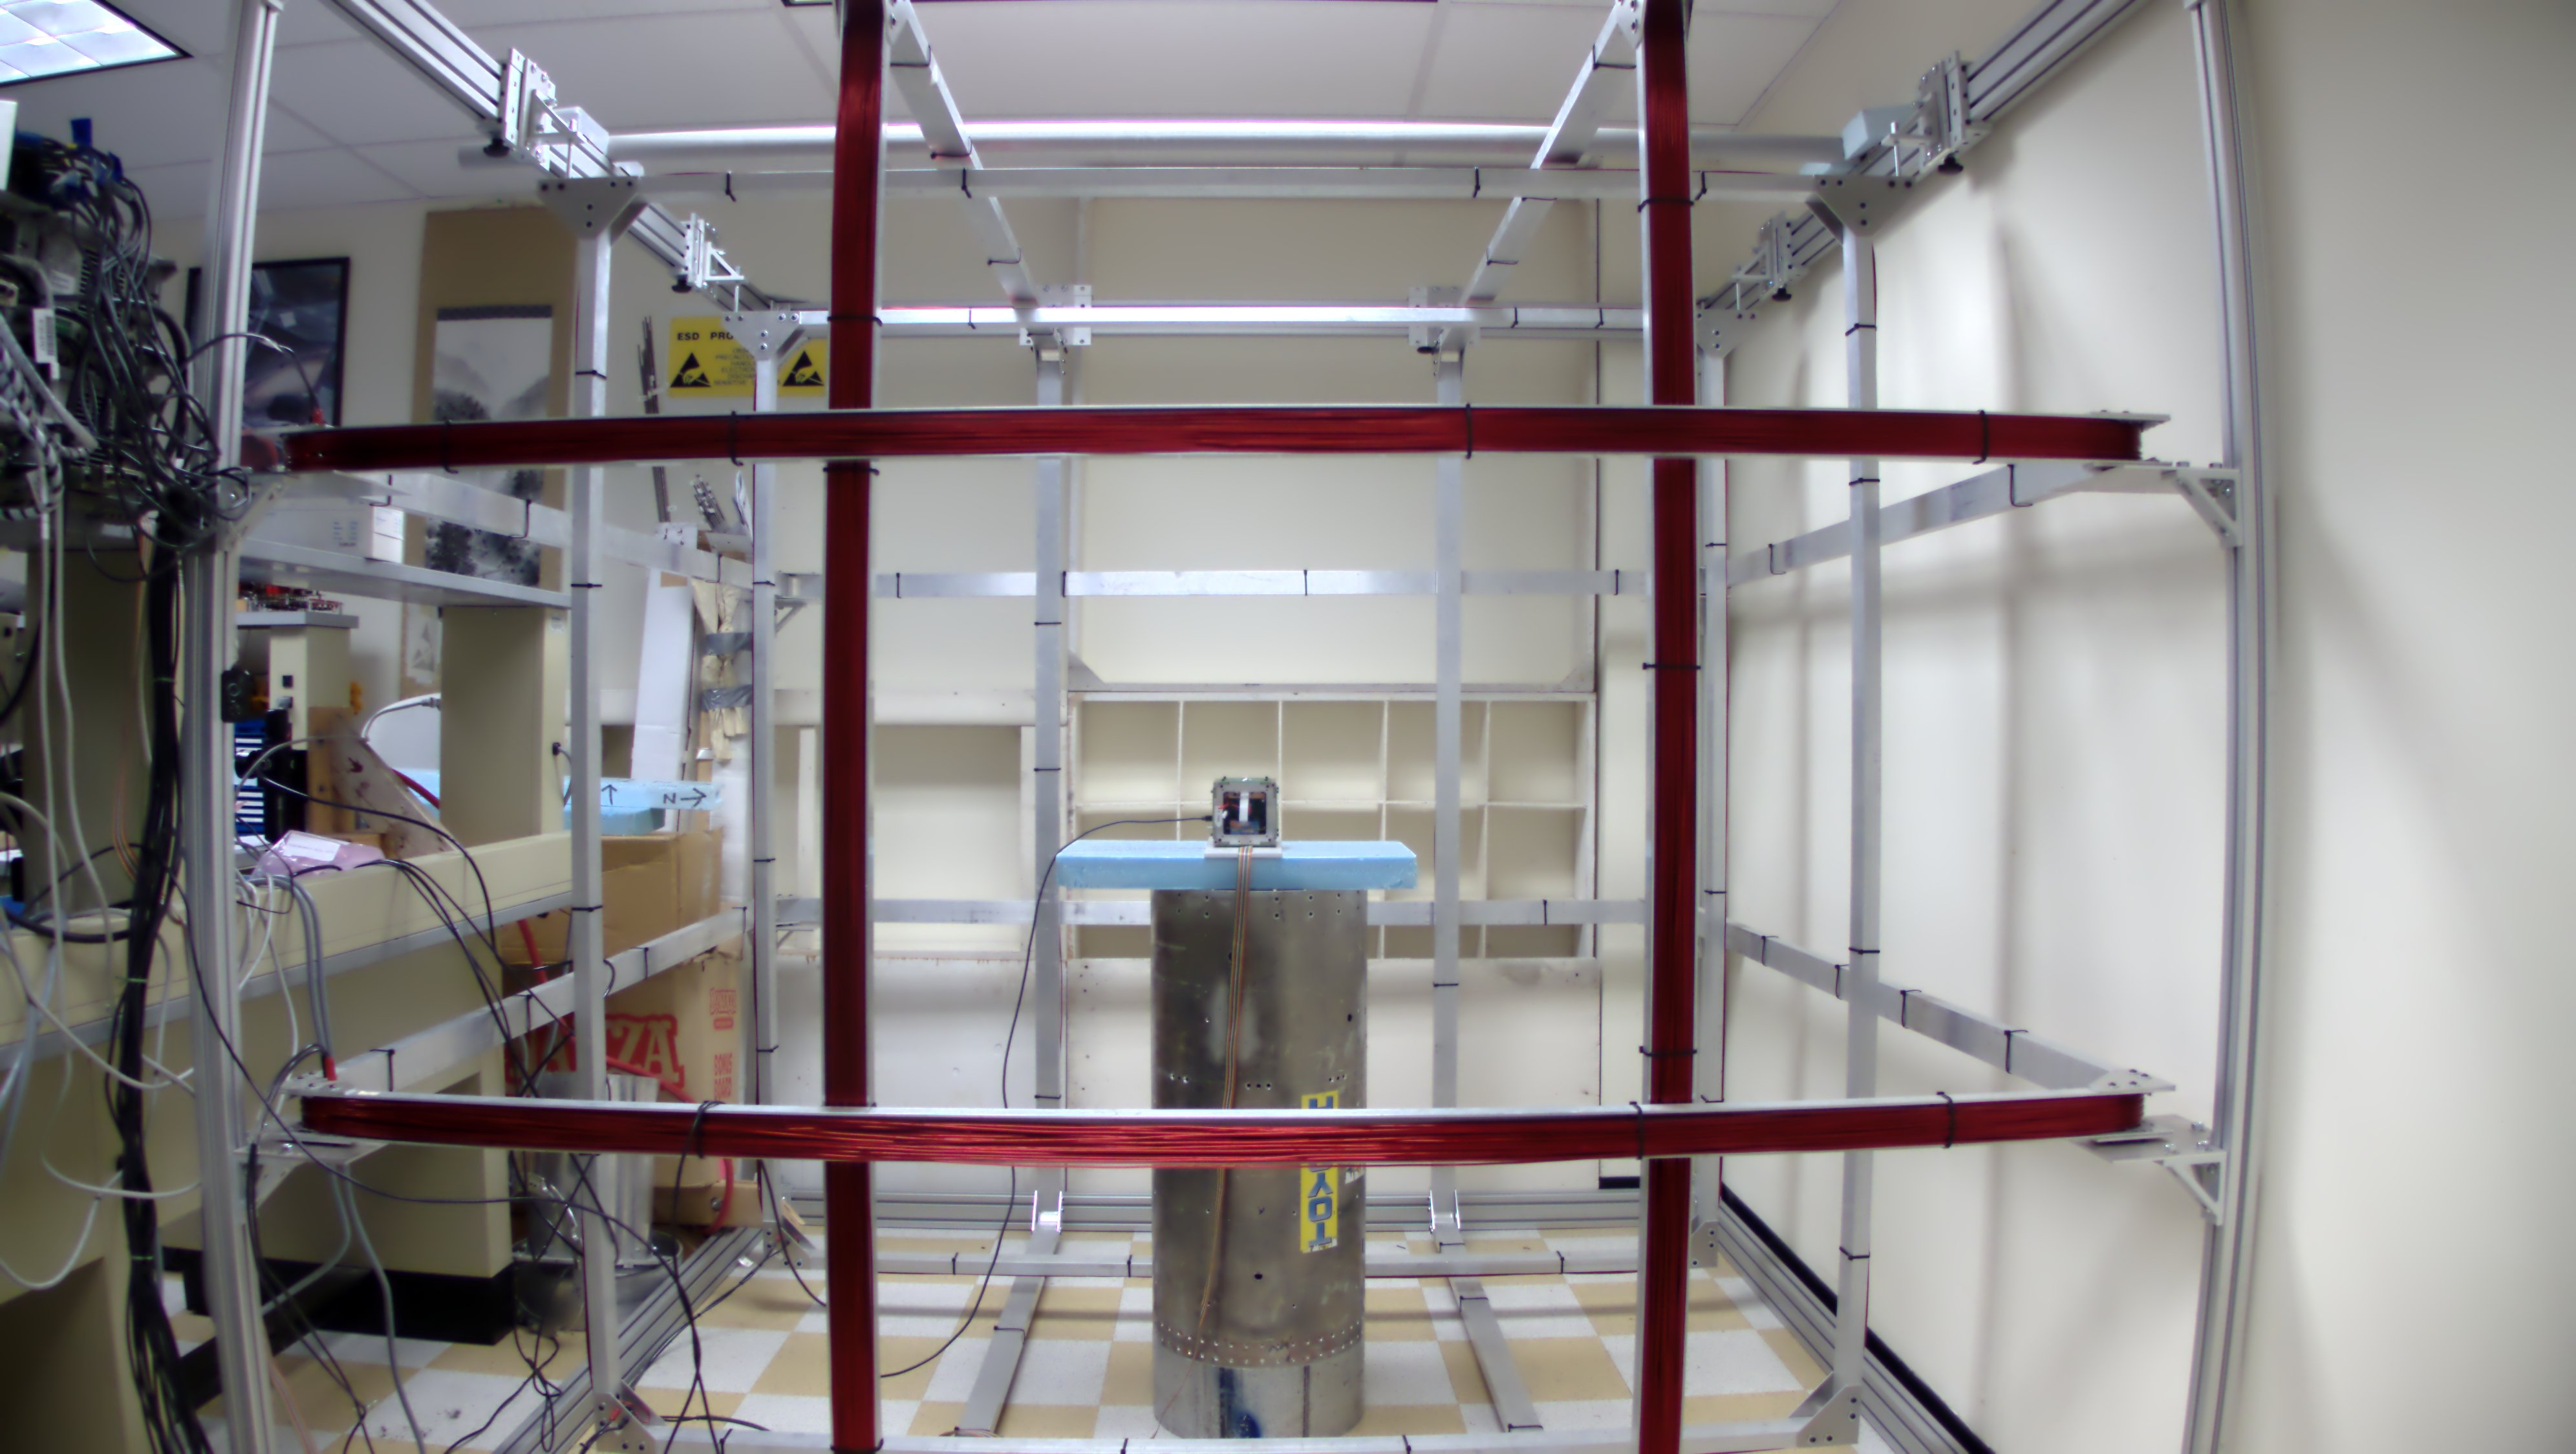
\includegraphics[width=\linewidth]{helmholtz-cage}
    \caption{The Helmholtz cage used for \acs{ACDS} testing}
    \label{fig:helmholtz}
\end{figure}

The coils are driven by a set of six Agilent E3633A power supplies as shown in \cref{fig:helmholtz-comp}. The power supplies have a maximum current of 20~A for output voltages less than 8~V or a maximum current of 10~A for output voltages of 20~V. The supplies are computer controlled with a \ac{GPIB} connection. 

An Alpha lab \#3AMG Milligauss Meter is used to measure the magnetic field of the Helmholtz cage. The meter is visible in \cref{fig:helmholtz-comp} to the left of the computer monitors. The Miligauss Meter has a digital display and an analog voltage output. The voltage output is read by a NI PCI-6010 Multifunction DAQ installed in the Helmholtz cage computer.

\begin{figure}[!ht]
    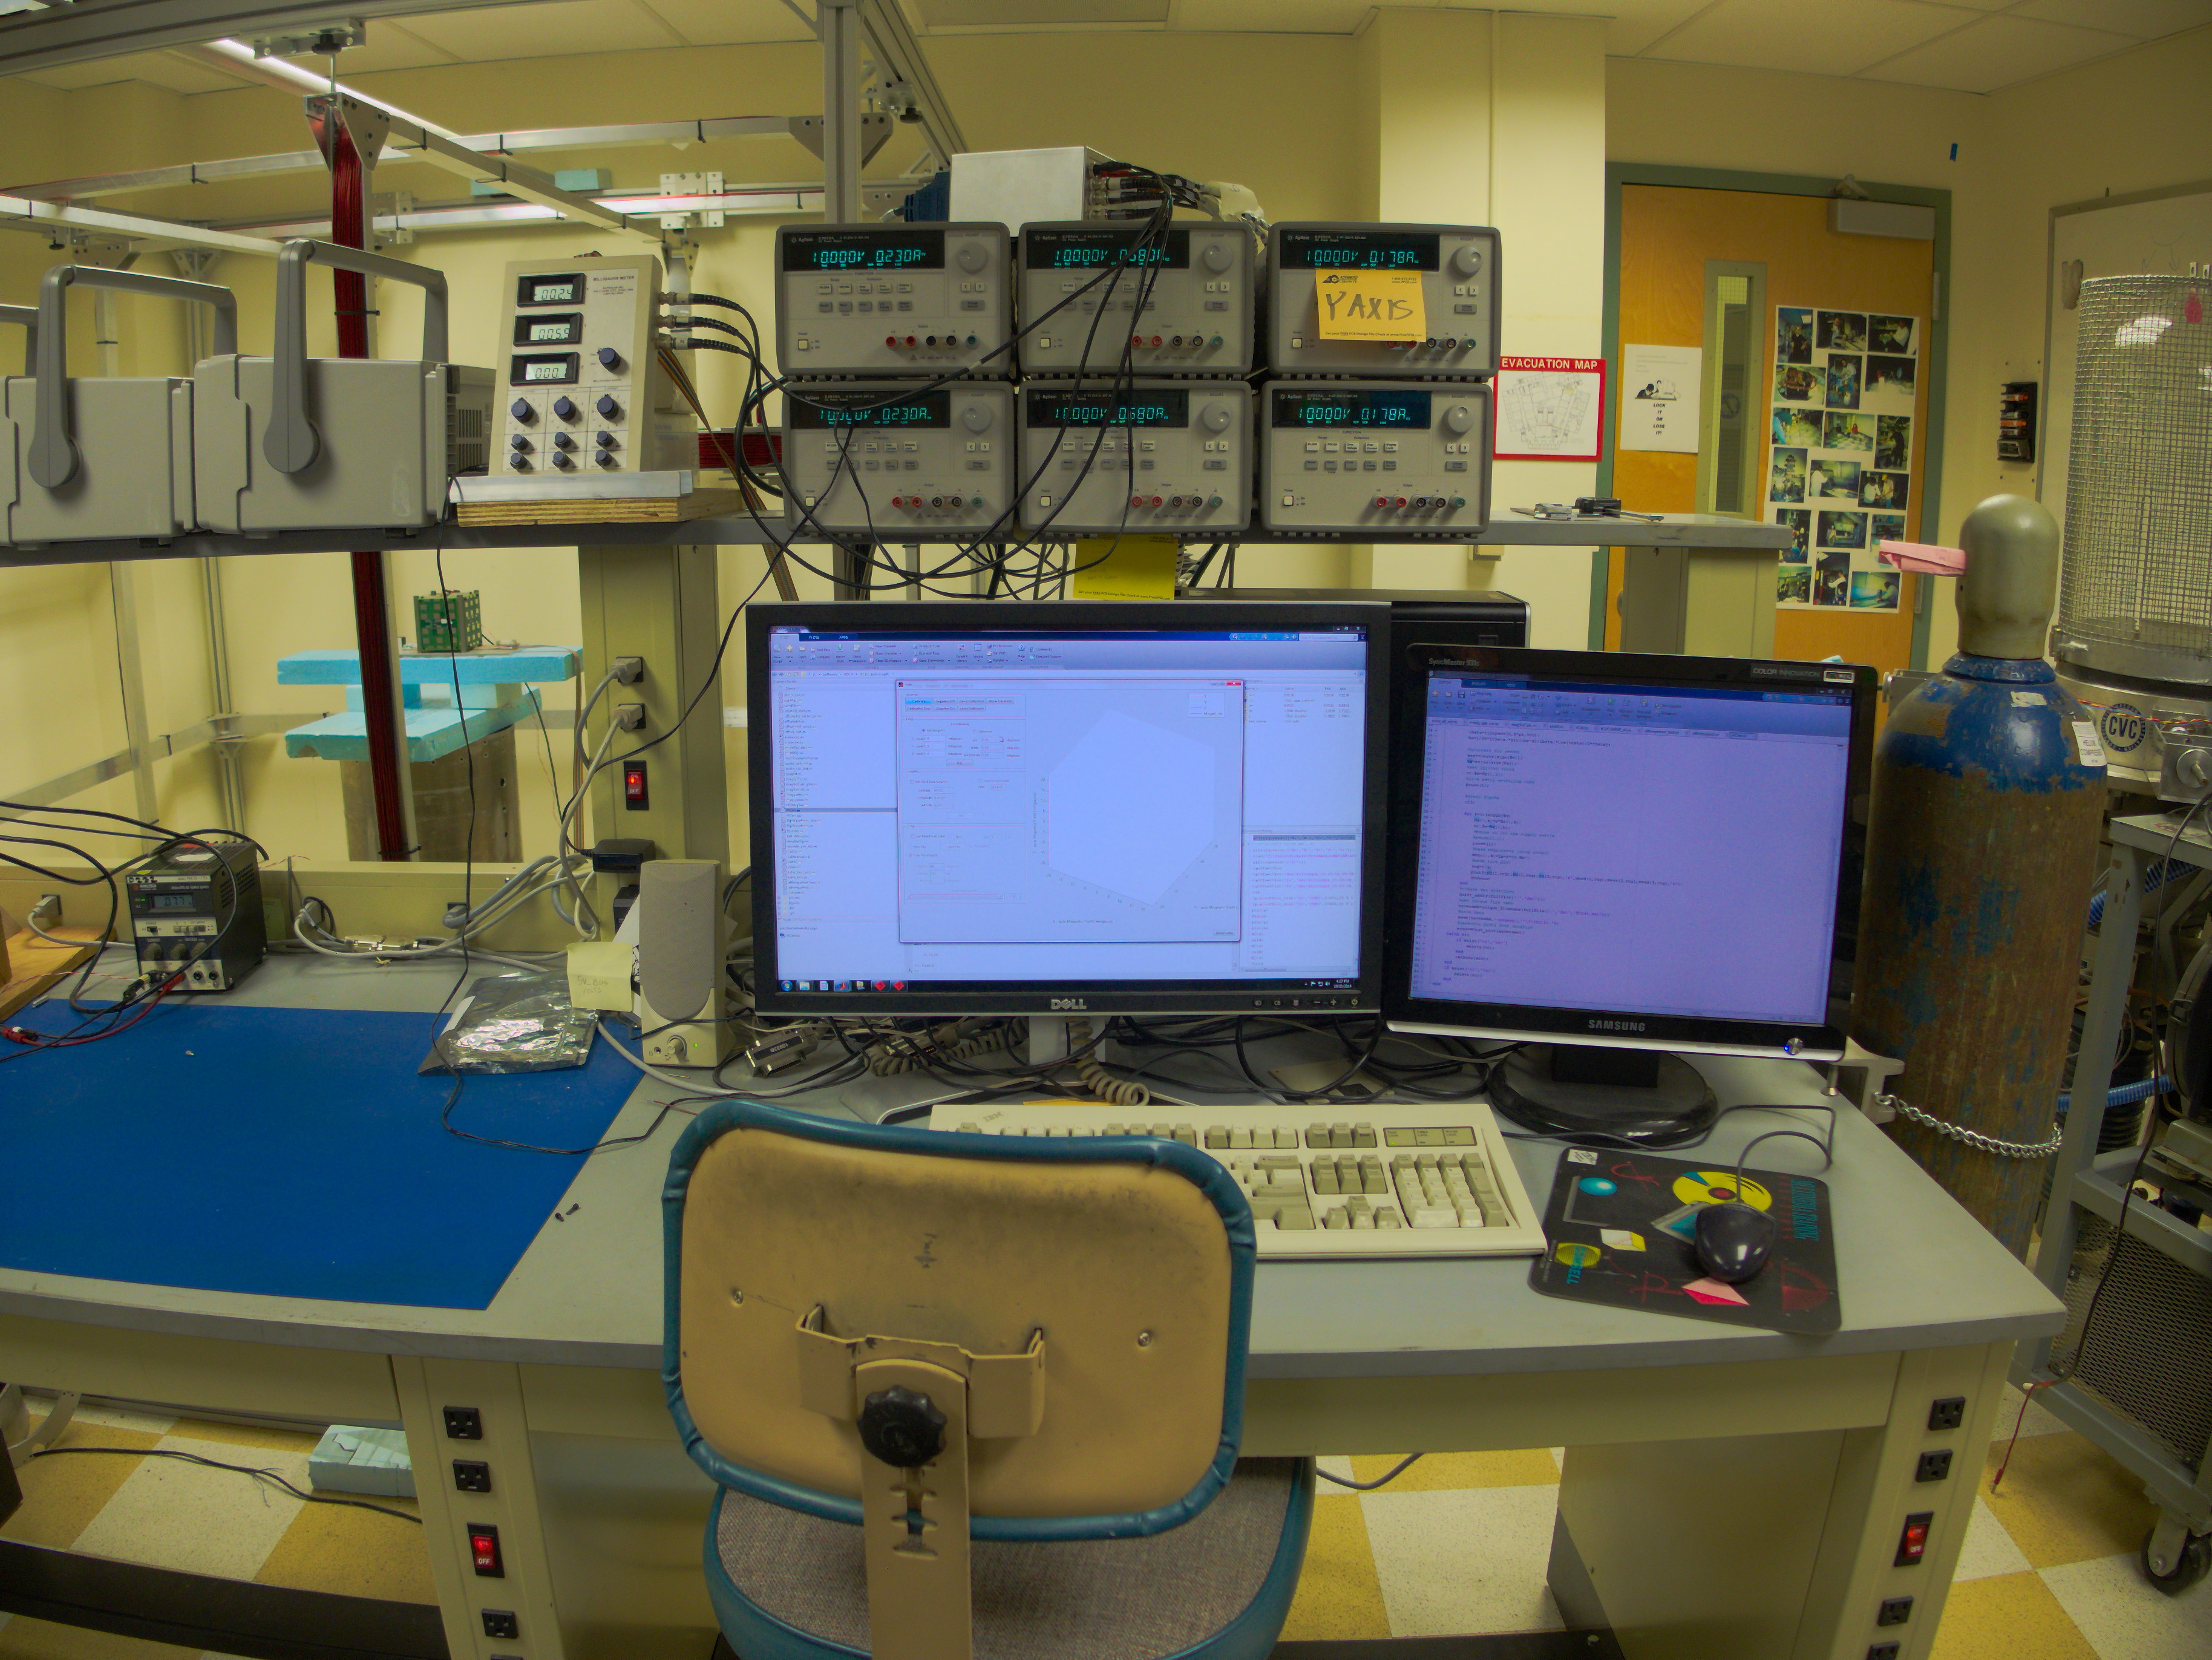
\includegraphics[width=\linewidth]{helmholtz-computer}
    \caption{The Helmholtz cage computer and power supplies}
    \label{fig:helmholtz-comp}
\end{figure}

\Cref{fig:hc-block} shows the block diagram of the Helmholtz cage.

\begin{figure}[!ht]
    \begin{tikzpicture}[node distance = 1cm, auto]
        \node[hardware] (coils) {Helmholtz Coils};
        \node[hardware] (dir)   {Direction Switch};
        \node[hardware] (ps)    {Power Supplies};
    \end{tikzpicture}
    \caption{Helmholtz cage software block diagram}
    \label{fig:hc-block}
\end{figure}


